\section{Estimation}
\subsection{Properties of estimation techniques}
\begin{figure}[h]
	\begin{center}
		\begin{subfigure}[b]{0.4\textwidth}
			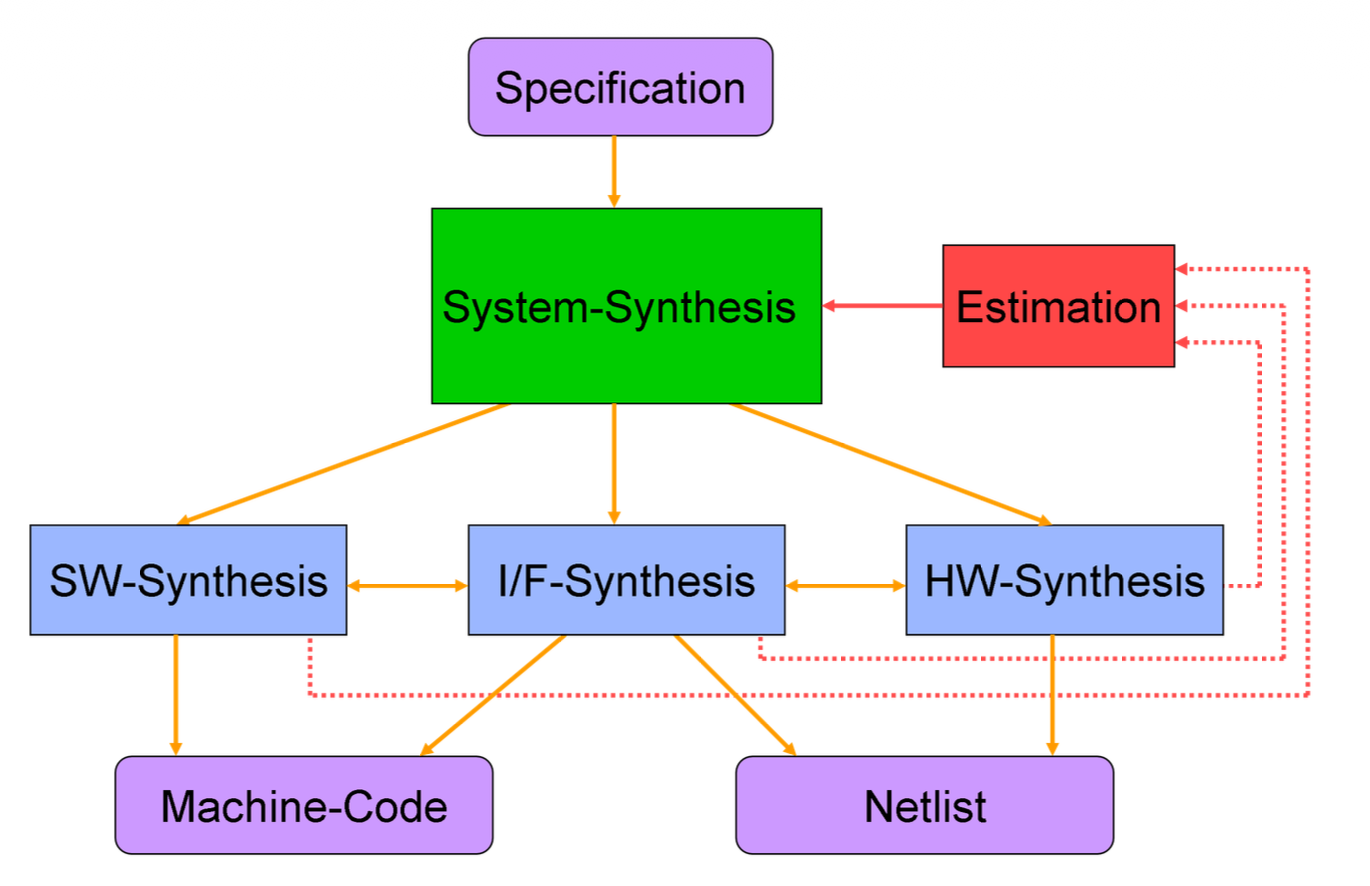
\includegraphics[width=\textwidth]{images/System_level_design.png}
			\caption{System-Level Design}
		\end{subfigure}
		\hfill
		\begin{subfigure}[b]{0.5\textwidth}
			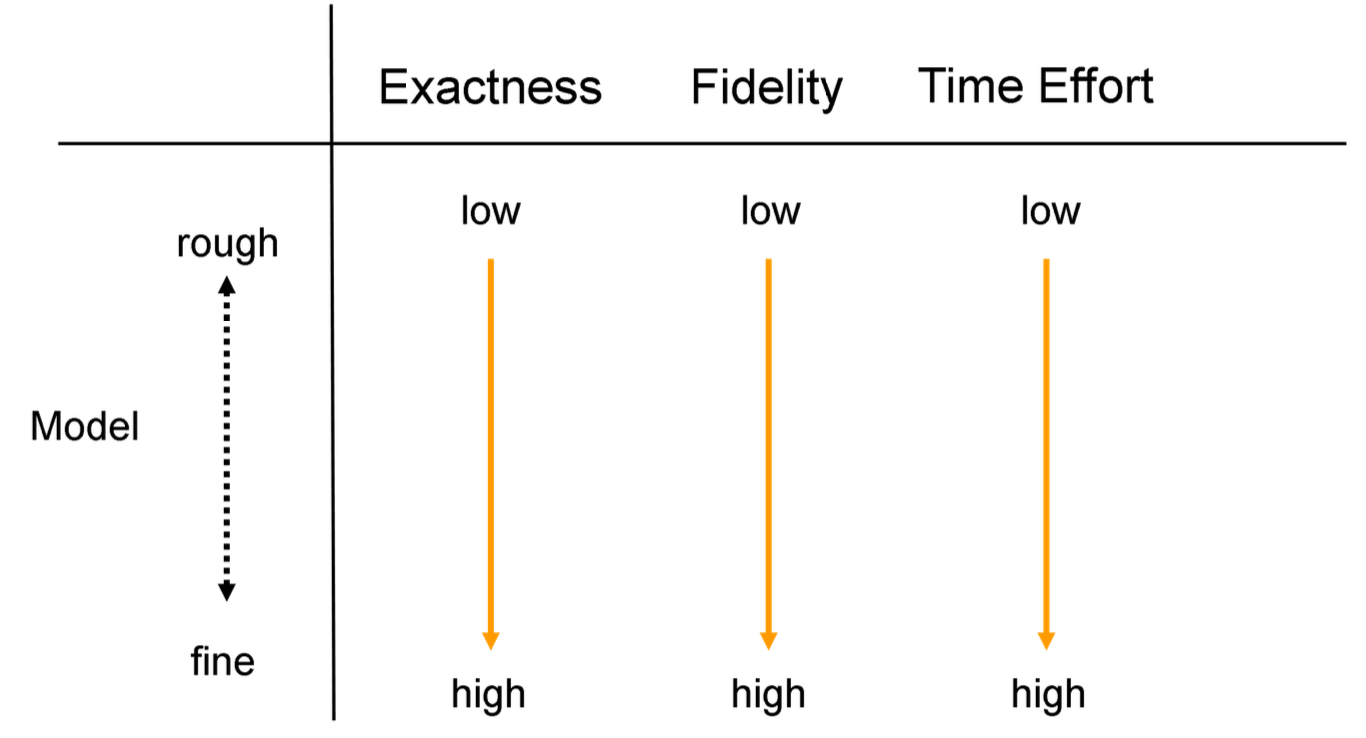
\includegraphics[width=\textwidth]{images/Estimation_properties.png}
			\caption{Properties of Estimation Techniques}
		\end{subfigure}
	\end{center}
\end{figure}

\subsubsection{Exactness}
Let $E(D)$ be an estimated and $M(D)$ the exact quality of an implementation $D$. The exactness $A$ is defined as
$$
	A=1-\frac{|E(D)-M(D)|}{M(D)}
$$

\subsubsection{Fidelity}
Let $D=\{D_1, \dots, D_n\}$ be a set of implementations. The fidelity $F$ of an estimation technique is the percentage of correct pairwise comparisons
$$
	F=100\cdot\frac{2}{n(n-1)}\cdot\sum_{i=1}^n\sum_{j=i+1}^n\mu_{i,j}
$$
\[
\mu_{i,j} =
\begin{cases}
1 & \text{if } 
\bigl(E(D_i) > E(D_j) \land M(D_i) > M(D_j)\bigr) \\
 & \quad \lor \bigl(E(D_i) < E(D_j) \land M(D_i) < M(D_j)\bigr) \\
 & \quad \lor \bigl(E(D_i) = E(D_j) \land M(D_i) = M(D_j)\bigr) \\
0 & \text{else}
\end{cases}
\]

\begin{figure}[h]
	\begin{center}
		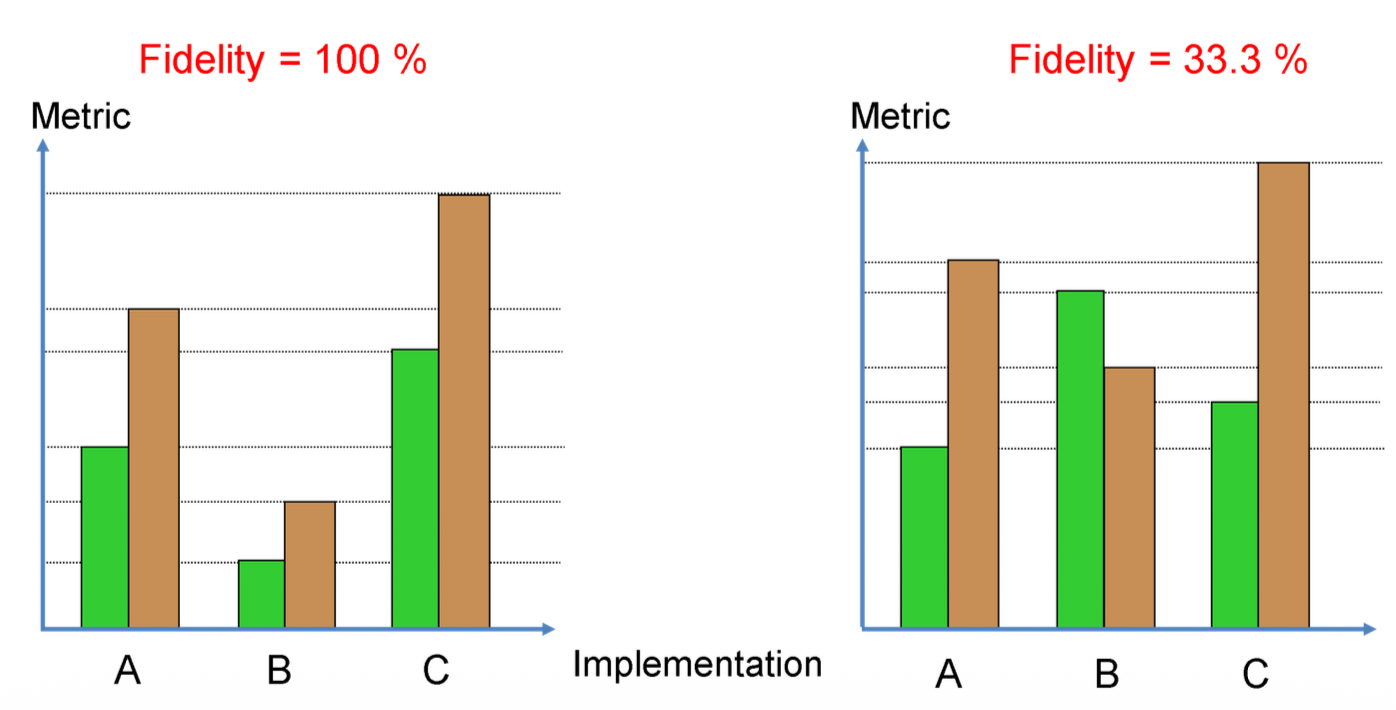
\includegraphics[width=0.5\textwidth]{images/Fidelity.png}
		\caption{Fidelity \\ Green: Estimation \\ Brown: Measurement}
	\end{center}
\end{figure}

\subsection{Qualities}
\begin{itemize}
	\item Performance
\begin{itemize}
	\item Hardware (clock period, latency, execution time, data rate)
	\item Software (execution time)
	\item Communication (maximal/average bit rate)
\end{itemize}
	\item Cost
	\item Further qualities
\begin{itemize}
	\item Power consumption
	\item Testability 
\end{itemize}
\end{itemize}

\subsubsection{HW Performance}
\begin{itemize}
	\item Clock period $T$ $\rightarrow$ Longest combinational path in circuits and technologie
	\item Latency $L$ $\rightarrow$ Execution time in clock cycles
	\item Execution time $\rightarrow$ $T_{ex} = T \cdot L$
	\item Data rate $R$ $\rightarrow$ Pipelining with $P$ steps of equal length: $R = \frac{P}{T_{ex}}$
\end{itemize}

\begin{figure}[h]
	\begin{center}
		\begin{subfigure}[b]{0.45\textwidth}
			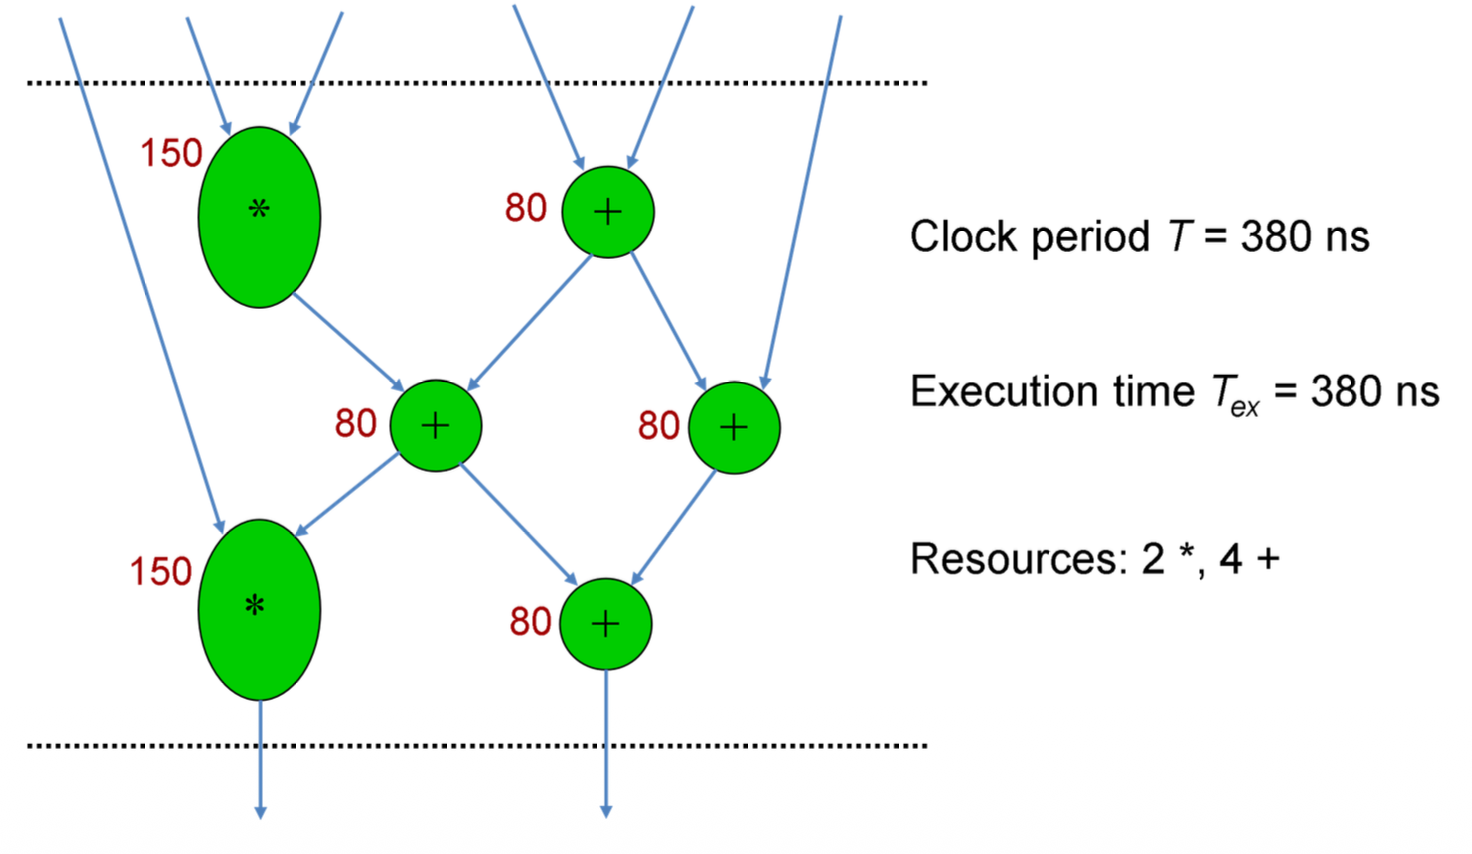
\includegraphics[width=\textwidth]{images/Performance_1.png}	
			\caption{Clock period $T = $ longest path }
		\end{subfigure}
		\hfill
		\begin{subfigure}[b]{0.45\textwidth}
			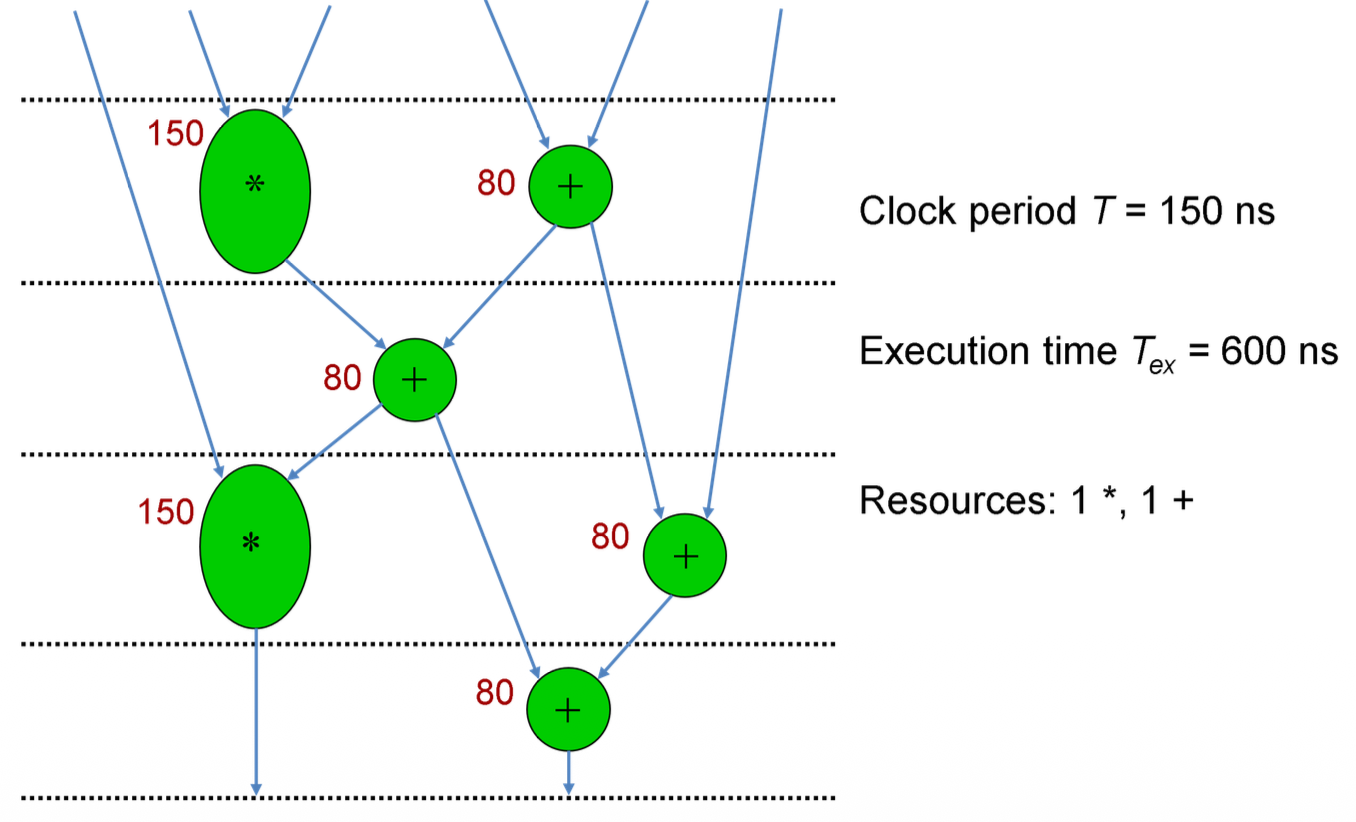
\includegraphics[width=\textwidth]{images/Performance_2.png}	
			\caption{Clock period $T=$ longest unit}
		\end{subfigure}
		\begin{subfigure}[b]{0.45\textwidth}
			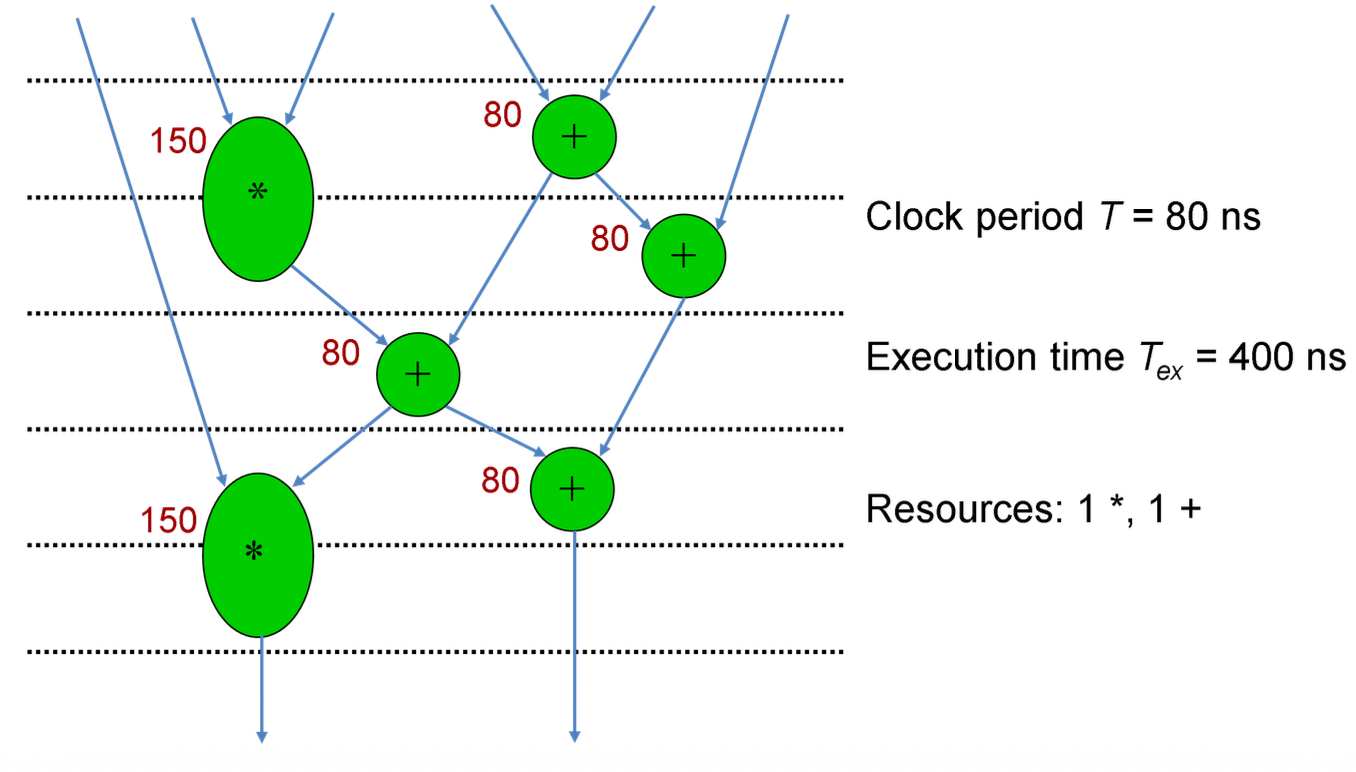
\includegraphics[width=\textwidth]{images/Performance_3.png}	
			\caption{Clock period $T=$ shortest unit}
		\end{subfigure}
		\hfill
		\begin{subfigure}[b]{0.4\textwidth}
			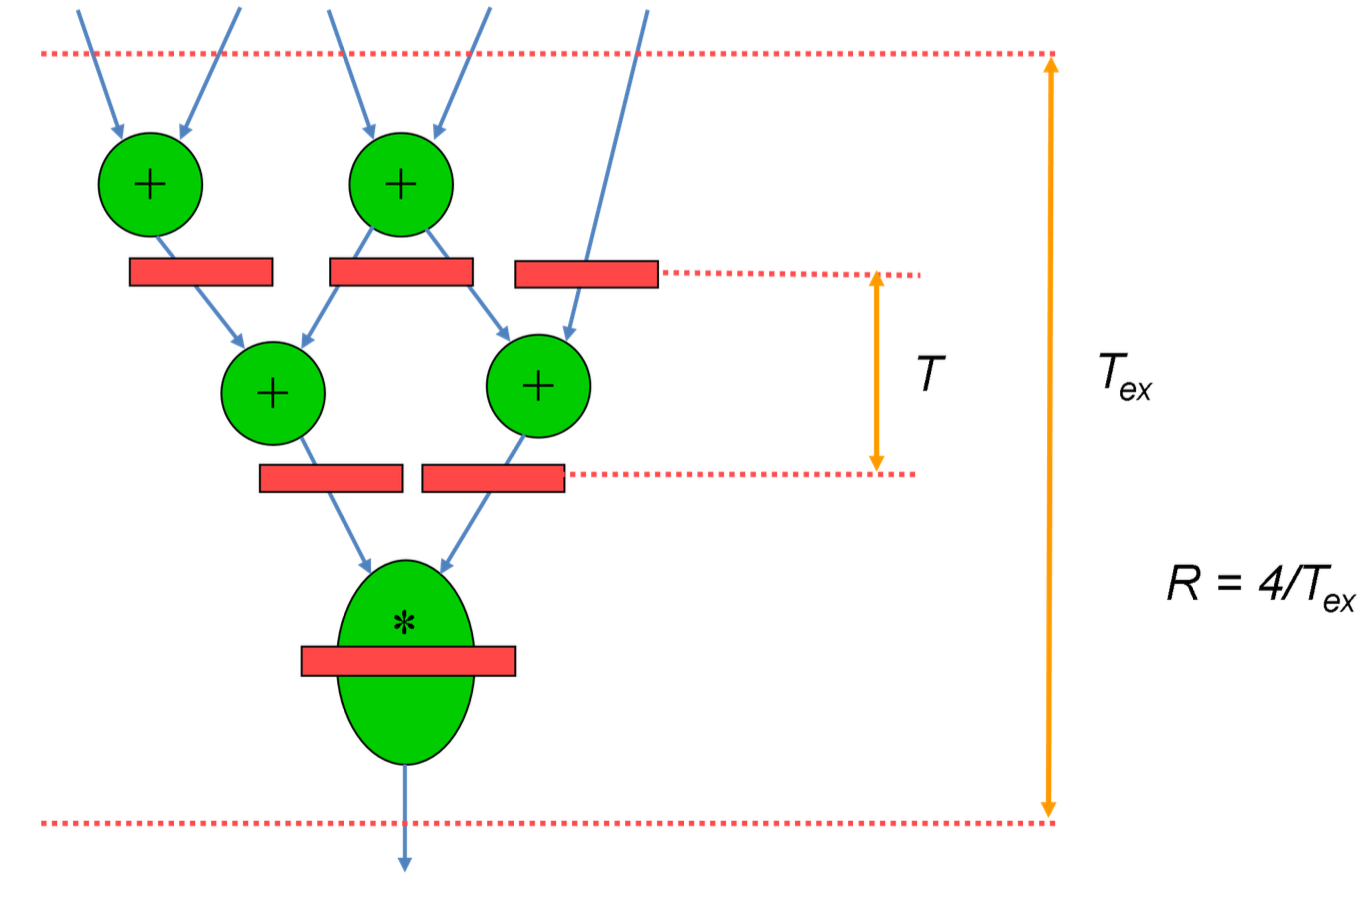
\includegraphics[width=\textwidth]{images/Performance_4.png}	
			\caption{Pipelining}
		\end{subfigure}
	\end{center}
\end{figure}

\subsubsection{SW Perfomance}
\begin{itemize}
	\item Execution time $T$
$$
	T = I_c \cdot CPI \cdot \tau = \frac{I_c\cdot CPI}{f}
$$
	\begin{itemize}
	\item $I_c$: Instruction count of a program
	\item $CPI$: Cycles per instruction (average)
	\item $\tau$: Clock period
	\item $f$: Clock frequency
\end{itemize}
	\item MIPS rate (million instructions per second)
$$
	MIPS = \frac{I_c}{\tau\cdot10^6} = \frac{f}{CPI\cdot10^6}
$$
	\item MFLOPS (million floating-point operations per second)
	\item MACS (million multiply and accumulates per second)
	\item MOPS (million operations per second)
\end{itemize}

\subsubsection{Communication Performance}
\begin{itemize}
	\item Model for communication time $T_{\text{comm}}$
$$
	T_{\text{comm}} = T_{\text{offset}} + \frac{\text{message size}}{\text{bitrate}}
$$
\begin{itemize}
	\item $T_{\text{offset}}$: time for initialization
	\item message size in Bit
	\item bitrate in Bit/sec
\end{itemize}
\end{itemize}

\subsubsection{Cost measures}
\begin{itemize}
	\item Hardware
\begin{itemize}
	\item Cost often proportional to area of circuit:
\begin{itemize}
	\item mm$^2$, $\lambda^2$
	\item number of transistors
	\item number of gates
	\item number of CLBs (FPGA)
\end{itemize}
	\item number of pins
\end{itemize}
	\item Software
\begin{itemize}
	\item Size of required program and data memory
\end{itemize}
\end{itemize}

\subsection{Estimation of hardware}
\begin{itemize}
	\item Given: functional units $v_k$ with delay del$(v_k)$
	\item Method of maximum operator delay:
$$
	T = \max_k(\text{del}(v_k))
$$
	\item Method for minimization of clock slack
\begin{itemize}
	\item Search in the interval $T_{\min} \dots T_{\max}$ for clock period $T$ producing the highest clock utilization
\end{itemize}
	\item ILP search
\end{itemize}

\subsubsection{Clock slack minimization}
\begin{itemize}
	\item Let occ$(v_k)$ denote the number of occurrences of operations of type $k$ and $|V_T|$ the number of different operation types. \\
		Then, the average slack is given as
		$$
			\text{avgslack}(T) = \frac{\sum_{k=1}^{|V_T|}(\text{occ}(v_k) \cdot \text{slack}(T, v_k))}{\sum_{k=1}^{V_T}\text{occ}(v_k)}
		$$
		And the clock utilization as
		$$
			\text{util}(T) = 1 - \frac{\text{avgslack}(T)}{T}
		$$
\end{itemize}

\subsection{Estimation of Software}
\begin{itemize}
	\item Execution time
\begin{itemize}
	\item Profiling: compilation and many test runs $\rightarrow$ statistical properties
	\item Estimation on the level of source-/intermediate-/target-code
	\item Important for applications with hard real-time constrains $\rightarrow$ Worst-Case Execution Time (WCET)
\end{itemize}
	\item Memory requirements
\begin{itemize}
	\item Program memory: compilation, estimation
	\item Data memory (only in case of static memory allocation)
\end{itemize}
\end{itemize}

\subsubsection{Worst-Case Execution Time (WCET)}
\begin{itemize}
	\item May not be determined by profiling
	\item Estimation using program path analysis techniques
\end{itemize}

\subsubsection{Program Path Analysis}
\begin{itemize}
	\item Delivers a WCET estimation that is greater or equal to WECT, but a good estimation is close to real WCET
	\item Processor model
\begin{itemize}
	\item Processor without interrupts and OS
\end{itemize}
	\item Programming model
\begin{itemize}
	\item No recursive function calls
	\item No pointer operations
	\item Loops musst have static bounds
\end{itemize}
\end{itemize}

\subsubsection{WECT Computation}
Let a program consist of $N$ basic blocks, each block $B_i$ having an execution time of $c_i$ and being executed $x_i$ times during program execution. Then, a WCET estimate may be calculated as
$$
	\text{WECT} = \max\{\sum_{i=1}^Nc_i\cdot x_i|\text{constraints}\}
$$

\subsubsection{Functional Constrains}
\begin{itemize}
	\item Defined by the programmer
\begin{itemize}
	\item Bounds of loop counter
	\item Knowledge of program context
\end{itemize}
	\item May be complex
\end{itemize}































